%!TEX root = ../Thesis.tex
\section{Feed forward Neural Network}
\label{sec:theory:ffnn}

Neural Machine Translation is based on the neural network framework. Modern networks are extremely complex and use rather advanced operations such as convolution, others use complex combinations of simpler operations such as the LSTM block \cite{deep-learning}. To give a short introduction to this framework the feed forward neural network (FFNN) is presented. This is the simplest type of network in the neural network family. As such it doesn't have much use for translation, but the more advanced neural networks can be seen as extensions of a feed forward neural network.

\subsection{The neuron}

The neuron is the main component of any neural network. Mathematically it is just a function which takes a vector and returns a scalar. It does this by a weighted sum of the inputs $\{ x_i \}_{i=1}^I$ and by adding a bias value $b$. The sum is then typically transformed using a non-linear function $\theta$.
\begin{equation}
a = \theta(z),\quad z = \sum_{i=1}^I w_{i} x_i + b
\end{equation}

The value $a$ is the output of the neuron and is called the \textit{activation}. In the past, the sigmoid function $\sigma(\cdot)$ and the hyperbolic tangent $\tanh(\cdot)$ function have been very popular \cite{bishop}, but recently the rectified linear unit (ReLU) $\theta(z) = \max(0, z)$ has gained popularity \cite{deep-learning}. If no non-linear function is applied then the identity function $\theta(a) = a$ is used.

\begin{figure}[H]
	\centering
	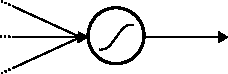
\includegraphics[scale=1]{theory/ffnn-neuron}
	\caption{Visual representation of a single neuron. The left arrows represent the input elements $\{ x_i \}_{i=1}^I$. The circle represents the function that returns the activation scalar $a$ (right arrow).}
\end{figure}

\subsection{The network}

A feed forward neural network is in its simplest form a \textit{multivariate non-linear regression model} constructed by combining neurons. Such a regression model can then be turned into a classification model by adding a softmax transformation \cite{the-elements-of-statistical-learning} to the output. By doing this each output value becomes the class probability $y_k = P(C_k | x)$.

\begin{figure}[h]
	\centering
	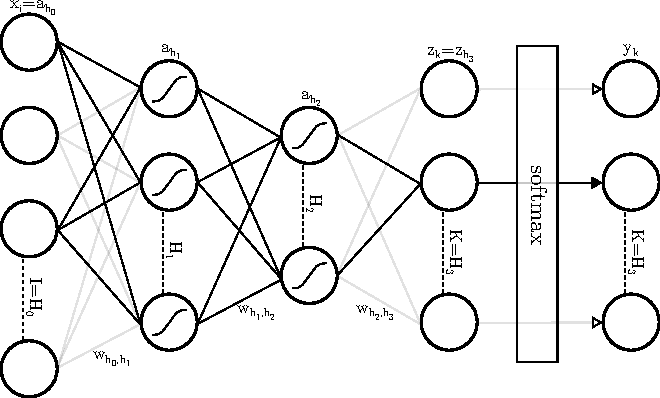
\includegraphics[scale=1]{theory/ffnn-network.pdf}
	\caption{Visual representation of a neural network with two hidden layers. Some lines are less visible, this is just a visual aid because the many connections can be difficult to look at.}
	\label{fig:theory:ffnn:network}
\end{figure}

The neural network in Figure \ref{fig:theory:ffnn:network}, have one input layer $x_i, i \in [1, I]$ and one output layer $y_k, k \in [1, K]$. This is the same for any neural network, what varies is the type of network (here a feed forward neural network) and the number of hidden layers (here two). The hidden layers are typically the layers that contain the non-linear transformation functions. If there are no hidden layers, the neural network is just a multi-class logistic regressor\cite{bishop}.

Because there is more than one neuron in each layer and many layers, the neuron index and layer index is denoted by the subscript. For example, a neuron output is denoted by $a_{h_{\ell}}$ for $h_{\ell} \in [1, H_{\ell}]$, where $h_{\ell}$ is the neuron index and $H_\ell$ is the number of neurons in layer $\ell$.

While diagrams like in figure \ref{fig:theory:ffnn:network} are useful for feed forward neural networks, they becomes too verbose for more complex networks. Instead each layer is just represented by a single block like in figure \ref{fig:theory:ffnn:network-block}.

\begin{figure}[h]
	\centering
	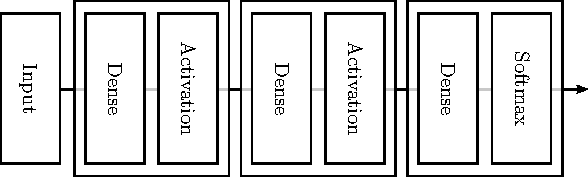
\includegraphics[scale=1]{theory/ffnn-network-block.pdf}
	\caption{Network block-diagram of the same network as shown in figure \ref{fig:theory:ffnn:network}.}
	\label{fig:theory:ffnn:network-block}
\end{figure}

In figure \ref{fig:theory:ffnn:network-block} the dense block represents a dense matrix multiplication, which is essentially just a neural network layer without the activation. This is then followed by an activation block, which in figure \ref{fig:theory:ffnn:network-block} is left unspecified for generality.

\subsection{Forward pass}

Calculation of the network output ($y_k$) is sometimes called the \textit{forward pass}, while the parameter estimation is sometimes called the \textit{backward pass}.

The \textit{forward pass} is simply calculated by applying the neuron function to all neurons in all layers. By defining $a_{h_0} = x_i$ the \textit{forward pass} can be generalized to any amount of hidden layers ($L$):
\begin{equation}
\begin{aligned}
a_{h_\ell} &= \theta(z_{h_\ell}), && \forall h_{\ell} \in [1, H_{\ell}], \ell \in [1, L] \\
z_{h_\ell} &= \sum_{h_{\ell-1} = 1}^{H_{\ell-1}} w_{h_{\ell-1}, h_{\ell}} a_{h_{\ell-1}} + b_{h_{\ell}}, && \forall \ell \in [1, L+1] \text{ where: } a_{h_0} = x_i, H_0 = I \\
\end{aligned}
\end{equation}

Note that the last layer $\ell = L + 1$ does not use the non-linear transformation function $\theta$, instead it uses the softmax function.
\begin{equation}
\begin{aligned}
y_k = \frac{\exp(z_k)}{\sum_{k'=1}^K \exp(z_{k'})}, && \forall k \in [1, K] \text{ where: } z_k=z_{h_{L+1}}, K = H_{L + 1}
\end{aligned}
\label{eq:theory:ffnn:y}
\end{equation}

The $z_k$ values are feed to the softmax function are often called \textit{logits}, because they are unnormalized log probabilities ($\exp(z_k) \propto y_k$), this has some advantages. For example, if one wants the most likely label given $\mathbf{x}$ one can just find the largest $z_k$ and thus skip the softmax, which can otherwise be quite expensive to calculate.

\subsection{Loss function}

Optimization of the parameters $w_{i,j}$ and $b_{j}$ requires a definition of a loss function. For classification it makes sense to maximize the joint probability of observing all the observations:
\begin{equation}
P(\mathbf{t} | \mathbf{x}, \mathbf{w}, \mathbf{b}) = \prod_{n=1}^N P(\mathbf{t}_n | \mathbf{x}_n, \mathbf{w}, \mathbf{b})  = \prod_{n=1}^N \prod_{k=1}^K P(C_{n, k} | \mathbf{x}_n, \mathbf{w}, \mathbf{b})^{t_{n, k}}
\end{equation}

Here $\mathbf{x}_{n}$ is the input vector for observation $n$, with a corresponding label vector $\mathbf{t}_n$. The label vector is an indicator vector constructed using 1-of-K encoding. The class probability $P(C_{n, k} | \mathbf{x}_n, \mathbf{w}, \mathbf{b})$ is $y_k$ from the \textit{forward pass} for observation $n$.

The logarithm is then used to create linearity and avoid numerical floating point issues. The sign is also changed such that it becomes a loss function:
\begin{equation}
- \ln\left(P(\mathbf{t} | \mathbf{x}, \mathbf{w}, \mathbf{b})\right) = - \sum_{n=1}^N \sum_{k=1}^K t_{n, k} \ln\left( P(C_{n, k} | \mathbf{x}_n, \mathbf{w}, \mathbf{b})\right)
\label{eq:theory:ffnn:long-loss}
\end{equation}

Because of the linearity in \eqref{eq:theory:ffnn:long-loss}, it makes sense to just consider the loss function for one data point, thus the $n$ index can be omitted. This gives the final loss function which is denoted by $\mathcal{L}$:
\begin{equation}
\mathcal{L} = - \sum_{k=1}^K t_{k} \ln\left( P(C_{k} | \mathbf{x}, \mathbf{w})\right) =  - \sum_{k=1}^K t_k \ln(y_k)
\label{eq:theory:ffnn:loss}
\end{equation}

The formulation in \eqref{eq:theory:ffnn:loss} is particularly useful as it allows for some numerical stability tricks, see Appendix \ref{appendix:numerical-stability:cross-entropy}

\subsection{Backward pass}

For the neural network, there is no closed form solution to optimizing the loss function. Instead, gradient-based optimization algorithms are used. Gradient-based optimization uses the derivatives of the loss function with respect to the parameters to iteratively optimize the parameters. This approach will be discussed in Section \ref{sec:theory:optimization}, for now the important part is to calculate the derivatives:
\begin{equation}
\begin{aligned}
\frac{\partial \mathcal{L}}{\partial w_{h_{\ell-1}, h_\ell}} \wedge \frac{\partial \mathcal{L}}{\partial b_{h_\ell}}, && \forall \ell \in [1, L + 1]
\end{aligned}
\label{eq:theory:ffnn:bprop-problem}
\end{equation}

For calculating the derivatives the \textit{error backpropagation} algorithm is used, this algorithm results in what is called the \textit{backward pass}.

The main trick in \textit{error backpropagation} is to define the partial derivative $\delta_{h_\ell}$, this is then used for bookkeeping and is what makes it feasible to calculate the derivatives.
\begin{equation}
\delta_{h_\ell} \defeq \frac{\partial \mathcal{L}}{\partial z_{h_\ell}}
\end{equation}

Using this definition the chain rule can be applied on \eqref{eq:theory:ffnn:bprop-problem}:
\begin{equation}
\begin{aligned}
\frac{\partial \mathcal{L}}{\partial w_{h_{\ell-1}, h_\ell}} &= \frac{\partial \mathcal{L}}{\partial z_{h_\ell}} \frac{\partial z_{h_\ell}}{\partial w_{h_{\ell-1}, h_\ell}} &&= \delta_{h_\ell} a_{h_{\ell-1}},&& \forall \ell \in [1, L+1],\quad a_{h_0} = x_i \\
\frac{\partial \mathcal{L}}{\partial b_{h_\ell}} &= \frac{\partial \mathcal{L}}{\partial z_{h_\ell}} \frac{\partial z_{h_\ell}}{\partial b_{h_\ell}} &&= \delta_{h_\ell},&& \forall \ell \in [1, L+1]
\end{aligned}
\end{equation}


Calculating $\delta_{h_\ell}$ is a bit more involved since $z_{h_\ell}$ affects more than one intermediate variable, but even so the chain rule can still be applied:
\begin{equation}
\begin{aligned}
\delta_{h_\ell} = \frac{\partial \mathcal{L}}{\partial z_{h_\ell}} &= \frac{\partial \mathcal{L}}{\partial a_{h_\ell}} \frac{\partial a_{h_\ell}}{\partial z_{h_\ell}} \\
&= \theta'(z_\ell) \sum_{h_{\ell+1}}^{H_{\ell+1}} \frac{\partial \mathcal{L}}{\partial z_{\ell+1}} \frac{\partial z_{\ell+1}}{\partial a_\ell} \\
&= \theta'(z_\ell) \sum_{h_{\ell+1}}^{H_{\ell+1}} \delta_{h_{\ell+1}} w_{h_\ell, h_{\ell+1}}, \forall \ell \in [1, L]
\end{aligned}
\label{eq:theory:ffnn:bprop}
\end{equation}

The last delta ($\delta_{h_{L+1}}$) is different but can still be calculated by using the chain rule (see appendix \ref{appendix:backward-pass:softmax} for how $\delta_{h_{L+1}}$ is derived).
\begin{equation}
\delta_{h_{L + 1}} = \delta_k = \frac{\partial \mathcal{L}}{\partial z_k} = \sum_{k'=1}^K \frac{\partial \mathcal{L}}{\partial y_{k'}} \frac{\partial y_{k'}}{\partial z_k} = y_k - t_k
\label{eq:theory:ffnn:bprop-delta-last}
\end{equation}

Using \eqref{eq:theory:ffnn:bprop-delta-last} and \eqref{eq:theory:ffnn:bprop} all $\delta_{h_\ell}$ for $\ell \in [1, L+1]$ can be calculated for a feed forward neural network with $L$ hidden layers. Note in particular how \eqref{eq:theory:ffnn:bprop-delta-last} is an error measure and this value is propagated back through the network by the $\delta_{h_\ell}$ equations in \eqref{eq:theory:ffnn:bprop}. This is why the method is called \textit{error backpropagation}.
